\subsubsection{Description / circuitry}
% Describe the tractive system active light and additional circuitry. Additionally, fill out the table:

Our TSAL system consists of two parts, LEDs and generator of frequency with power-switch. Generator is in ECUB protected by fuse. The waveform is generated with a 555-based circuit. The TSAL uses pairs of anti-parallel LEDs and is connected with two wires. Color of the light is decided by the polarity of the driving voltage. The following table shows the operation mode depending on conditions C1, C2:

% dodat tabulku

EV4.12.1 is achived by U4 in Figure 21 - TSAL HV part schematic comparing the voltage on R59 with 3v3 reference. MHVout is connected to output connector of accumulator. O4 carries the information about HV presence to LV system and enables power to TSAL by opening Q5.

\begin{figure}[H]
	\centering
	\includegraphics[width=\textwidth]{./img/TSAL-ECUB-schematic.png}
	\caption{Schematic of generator for TSAL.}
	\label{fig:TSAL-ECUB-schematic}
\end{figure}

\begin{table}[H]
	\centering
	\caption{Parameters of the TSAL}
	\begin{tabularx}{\textwidth}{|X|X|}
		\hline
		Supply voltage: & +/- 24VDC \\[\TableSize]
		\hline
		Max. operational current: & 300mA \\[\TableSize]
		\hline
		Lamp type & Bi-color LED \\[\TableSize]
		\hline
		Power consumption: & 7.2 W \\[\TableSize]
		\hline
		Brightness & 124 Lumen (red), 29 Lumen (green) \\[\TableSize]
		\hline
		Frequency: & 3.96Hz \\[\TableSize]
		\hline
		Size (length x height x width): & 128mm x 20mm x 32mm \\[\TableSize]
		\hline
	\end{tabularx}%
	\label{tab:TSAL}%
\end{table}%

\begin{figure}[H]
	\centering
	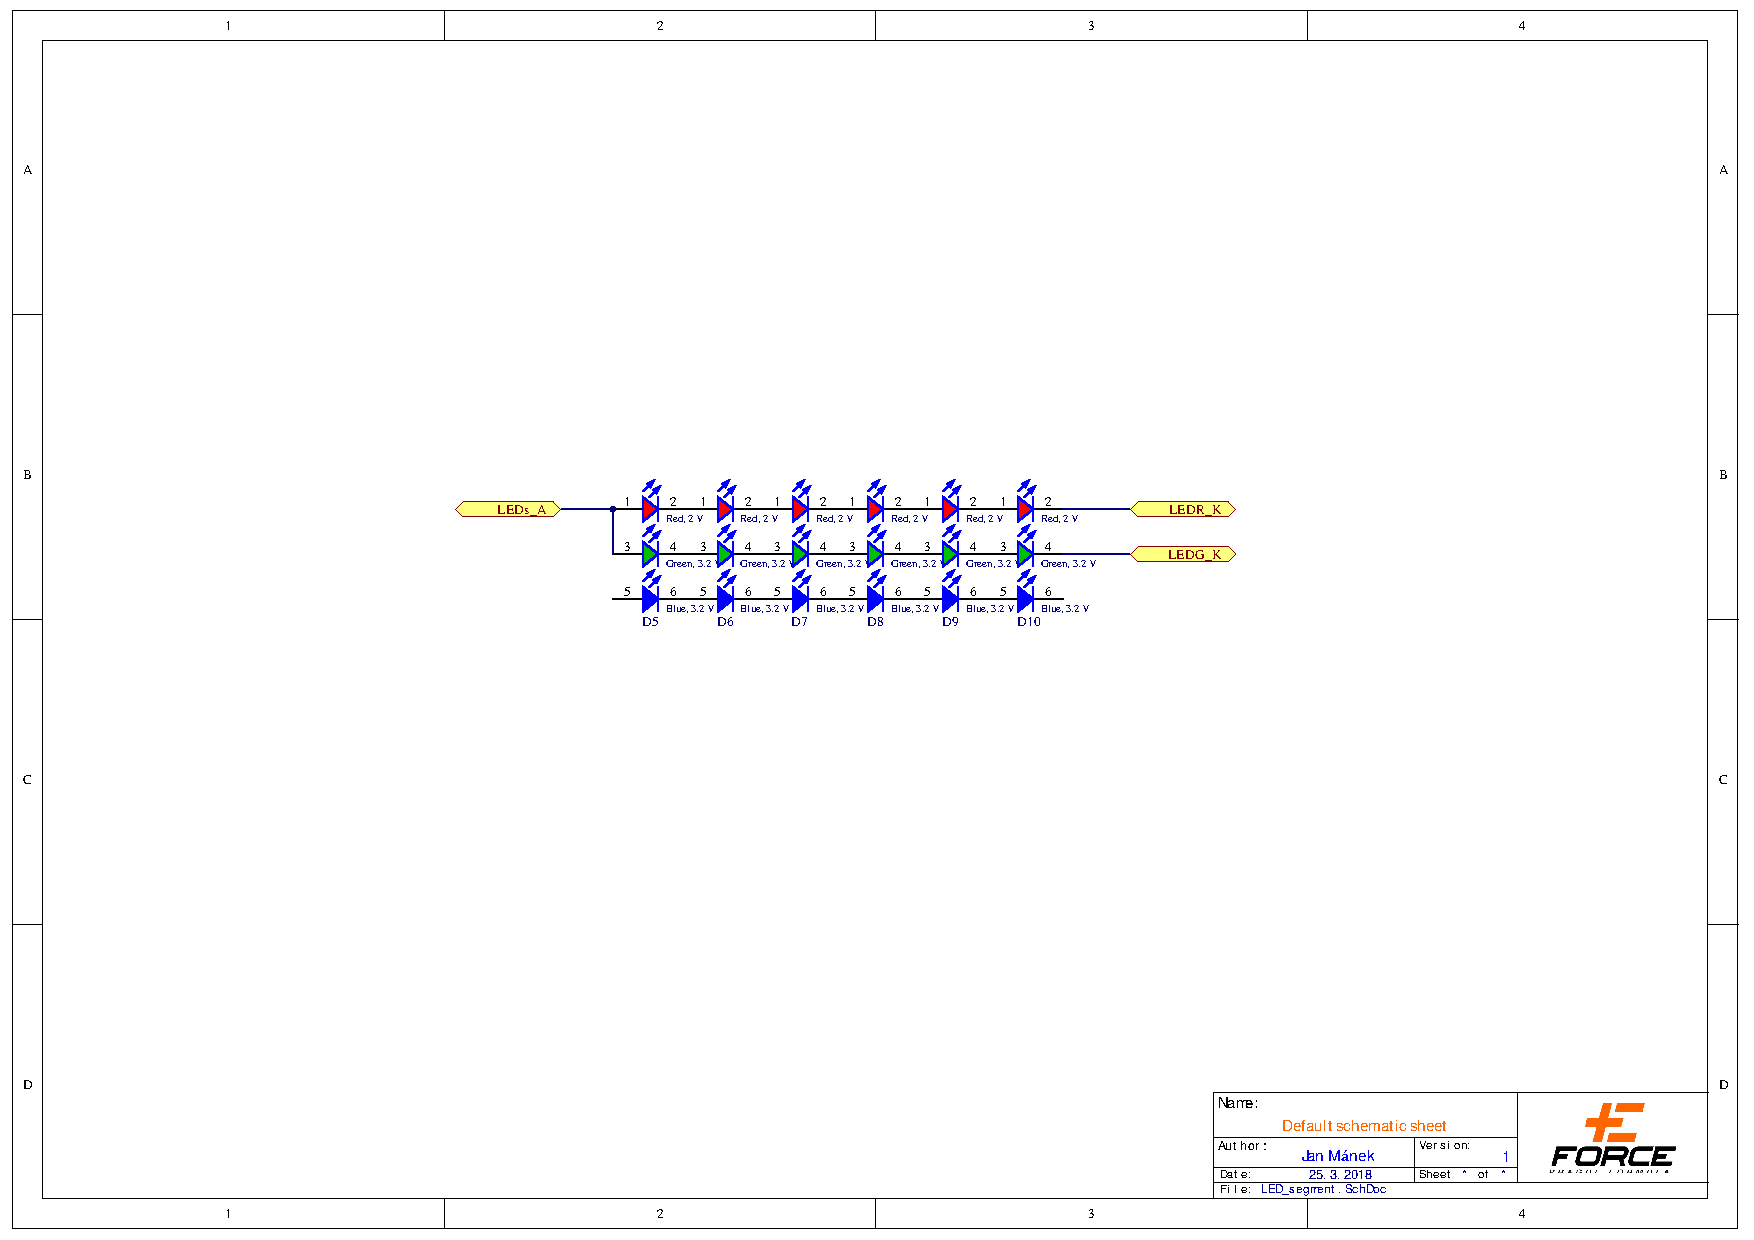
\includegraphics[width=\textwidth,trim={6cm 10cm 6cm 7cm},clip]{./img/TSAL-schematic.pdf}
	\caption{TSAL schematic.}
	\label{fig:TSAL-schematic}
\end{figure}

\begin{figure}[H]
	\centering
	\includegraphics[width=\textwidth]{./img/tsal-hv.jpg}
	\caption{TSAL HV part schematic.}
	\label{fig:TSAL-HV}
\end{figure}

\paragraph{Explanation of TSAL circuit}

Left top corner of \ref{fig:TSAL-HV} (input marked as HV-Viper) is directly connected to the output HV pins of ACP. The circuit is designed with STM chip „VIPER16HN“. It behaves as normal fly-back, with input voltage range from 50V up to 500V. Output of flyback is used to directly power the TSAL. ACP indication led is powered from primary side of transformer. To ensure correct behaviour, we also measure and compare input voltage (using U12A OAMP as comparator with little hysteresis), to enable output (Q36 \& Q33) only if input voltage is >=60VDC.

\begin{figure}[H]
	\centering
	\includegraphics[width=\textwidth]{./img/tsal-position.jpg}
	\caption{TSAL enable scheme}
	\label{fig:TSAL-enable}
\end{figure}

Function of circuit on \ref{fig:TSAL-enable} is that the TSAL is enabled even when the 60VDC limit is not reached, but the AIR is closed nonetheless. In such state, the TSAL is enabled by signal AIR\_EN. The circuit is powered by MAIN24 power (which is equal to the 24V enabled by GLVMS) or by the TSAL\_ACP-EN power signal from the Viper-TSAL schematic (\ref{fig:TSAL-ACPindicator}) below.

\begin{figure}[H]
	\centering
	\includegraphics[width=\textwidth]{./img/tsal-indicator.jpg}
	\caption{ACP indication LED wiring}
	\label{fig:TSAL-ACPindicator}
\end{figure}

%schema z backu
\subsubsection{Wiring/cables/connectors}
\iffalse Describe wiring, show schematics, describe connectors and cables used and show useful data regarding the wiring.  Include gauge, voltage and temperature rating of wiring used and any fuses or other overcurrent protection used.\fi

LEDs are supplied from ECUB (by Harness\_D by connector D1) by 2-wire low voltage cable (\ref{fig:TSAL-wiring}).

\begin{figure}[H]
	\centering
	\includegraphics[width=\textwidth,]{./img/tsal-wiring.jpg}
	\caption{Wiring TSAL from ECUB}
	\label{fig:TSAL-wiring}
\end{figure}

\subsubsection{Position in car}
%Provide CAD-renderings showing the relevant parts. Mark the parts in the rendering, if necessary.
TSAL is placed under the main roll hoop, see \ref{fig:TSAL-position}

\begin{figure}[H]
	\centering
	\includegraphics[width=\textwidth,trim={3cm 11cm 2cm 1cm},clip]{./img/tsal-position.pdf}
	\caption{TSAL position.}
	\label{fig:TSAL-position}
\end{figure}